\subsection{Asunciones previas}
Como se ha indicado en la sección del contexto de la empresa
\ref{context:company}, su especialidad son los desarrollos web y de
aplicaciones móviles. Es por ello que desde el principio se habló de que el
desarrollo de la \gls{api}, sería un desarrollo web.

\subsubsection{Tecnología propuesta}
Debido a que la empresa cuenta con trabajadores que ya realizaron proyectos con
una tecnología específica, se me pidió que usara la susodicha tecnología para
así facilitar la modificación, adaptación o corrección de errores una vez el
proyecto estuviera finalizado. La tecnología propuesta, por lo tanto, fue
Symfony.

\subsection{Frameworks utilizados en la aplicación}

\subsubsection{Symfony}
Symfony es un \glslink{webframework}{framework} escrito en \gls{php} y
organizado en \textit{bundles} o paquetes que permite realizar desarrollos web
disminuyendo la \gls{accidentalComplexity}. De hecho, una de las
características de Symfony es que absolutamente todo se organiza en paquetes.
Incluso el propio \glslink{webframework}{framework}, es un paquete. Otro de los
puntos fuertes de Symfony es que gracias a cómo ha sido desarrollado, fuerza a
programar siguiendo buenas prácticas y patrones conocidos, que hacen que la
calidad del código aumente.

\subsubsection{API Platform}
\label{tech:apiplat}
API Platform es a su vez otro \glslink{webframework}{framework} que está
diseñado especialmente para funcionar sobre Symfony, y que facilita la creación
de \gls{api}s. Una de sus características más llamativas es que una vez
definidas las entidades del dominio en clases \gls{php}, API Platform genera
automáticamente operaciones \gls{crud}. Otras de las funcionalidades destacables
que tiene, son entre otras:

 \begin{itemize}
    \item Soporte para diferentes formatos: XML, JSON, CSV y YAML.
    \item Soporte para la \glslink{semanticweb}{web semántica}: JSON-LD y HAL.
    \item Soporte para \gls{api}s \gls{hateoas}.
    \item Generación automática de documentación para las operaciones de la
        \gls{api} mediante \gls{swaggerui}.
    \item Paginación de resultados.
    \item Filtros de resultados.
 \end{itemize}

\subsection{Librerías destacables utilizadas en la aplicación}
Las dependencias de librerías externas en \gls{php} se suelen gestionar con
\textit{Composer}: este programa utiliza un fichero JSON que va llevando cuenta
de las dependencias requeridas y en qué versión se instalaron, de forma que los
proyectos no necesitan incluir dichas librerías cuando se despliegan o cuando
los diferentes miembros que contribuyen en él hacen acopio del código fuente.
Con un simple comando, \textit{Composer} leerá las dependencias requeridas y
las descargará desde el repositorio localizado en \url{https://packagist.org/}.
El formato en el que se recogen las librerías sigue el patrón
\textit{vendor/package}, y es el que utilizaré para describir algunas de las
librerías más interesantes utilizadas en el proyecto.

\subsubsection{api-platform/core}
El núcleo de API Platform. Esta librería es la que facilita las funcionalidades
indicadas en la sección de \glslink{webframework}{frameworks} \ref{tech:apiplat}
.

\subsubsection{symfony/http-foundation}
Define una capa orientada a objetos para la especificación HTTP
\cite{symfony_httpfound}, la cual tiene como finalidad englobar las variables
y funciones que \gls{php} utiliza para gestionar y manipular las peticiones
recibidas y las respuestas generadas\cite{symfony_httpfound_two}. Por ejemplo,
en el siguiente bloque de código, se muestra cómo las variables globales
\textemdash como \textit{\$\_GET} o \textit{\$\_POST}\textemdash que en un
principio habría que gestionar individualmente, se agrupan en cambio en un único
objeto de tipo \textit{Request} mucho más manejable.

\begin{minted}[linenos=true]{php}
<?php

use Symfony\Component\HttpFoundation\Request;

$request = Request::createFromGlobals();

$request = new Request(
    $_GET,
    $_POST,
    array(),
    $_COOKIE,
    $_FILES,
    $_SERVER
);
\end{minted}

La librería también permite acceder a la sesión, a las cabeceras enviadas,
enviar una respuesta, establecer \glslink{cookie}{cookies}, redireccionar
al usuario y múltiples funcionalidades más.

\subsubsection{symfony/http-kernel}
Esta librería se encarga de transformar la petición del usuario recibida en
una respuesta. Para ello, se sirve de el sistema de eventos que tienen
implementado \textemdash \textit{symfony/event-dispatcher}\textemdash el cual
va disparando varios eventos en cada fase de un proceso que se ilustra en la
siguiente ilustración:

\begin{figure}[h]
    \center
    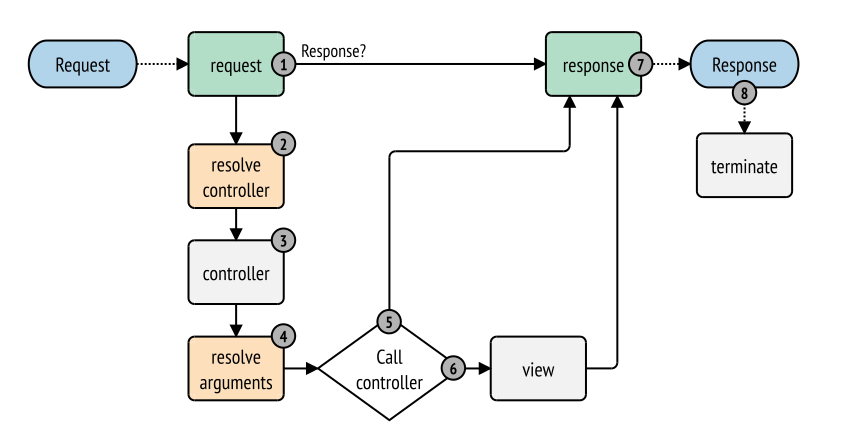
\includegraphics[scale=0.3]{img/http-workflow}
    \caption{Diagrama del proceso de transformación de una petición a una
        respuesta.}
    Fuente: \url{https://symfony.com/doc/current/components/http_kernel.html}
\end{figure}

Cada número representa un paso del proceso, y algunos de estos pasos dispararán
eventos. Al igual que existen eventos, también existen suscriptores a dichos
eventos, que básicamente esperan a que un evento de un tipo determinado se
dispare para realizar una serie de acciones.

\begin{enumerate}
    \item El evento \textit{kernel.request} tiene como objetivo añadir más
        información a la petición \textemdash por ejemplo después de determinar
        en qué idioma debería de darse la respuesta\textemdash, inicializar
        partes del \glslink{webframework}{framework} o crear una respuesta
        inmediatamente y finalizar el proceso: como por ejemplo cuando el
        usuario no tiene la autorización pertinente.
    \item El siguiente paso es averiguar qué controlador ha de llamarse para
        que se ejecute la lógica de negocio acorde a esa respuesta. Esto se
        determina gracias a la información que se extrae de la petición, y a la
        que el programador proporciona al \glslink{webframework}{framework} en
        forma de ciertas directrices como puede ser emparejar una ruta con
        un controlador. Ejemplo: \textit{\"Cuando una petición se realice a la
        ruta /hello/world, se ejecutará la función HelloWorld() del controlador
        HelloWorldController"}.
    \item El evento \textit{kernel.controller} tiene como objetivo preparar la
        ejecución del controlador, ya sea inicializando ciertas partes del
        \glslink{webframework}{framework} o incluso permitiendo que un
        suscriptor cambie el controlador que se va a ejecutar.
    \item En este punto se determinan los argumentos y los valores que han de
        pasarse al controlador. Las formas más comunes de determinarlo suelen
        ser mediante un identificador en la ruta\\ \textemdash
        \textit{/hello/world/argumento1/argumento2}\textemdash, la indicación
        que el programador da para obtener el argumento y finalmente pasando
        directamente la petición al controlador, donde el programador la
        procesará y extraerá los argumentos que le interesen.
    \item Aquí se llama al controlador y se aplica la lógica de negocio
        pertinente según lo que el programador haya programado. En el caso de
        que el controlador devuelva una respuesta, directamente se salta al
        último paso. En caso contrario, se realiza un paso más.
    \item El evento \textit{kernel.view} transforma un resultado de un
        controlador en una respuesta. Aquí es donde suele entrar en juego la
        capa de visualización. Por ejemplo: el controlador devuelve una serie
        de valores que después se insertan en la página correspondiente que
        haya que devolver al usuario, como puede ser el nombre de usuario del
        usuario que realizó la petición.
    \item Finalmente se dispara el evento \textit{kernel.response}, que permite
        a los distintos suscriptores modificar la respuesta antes de que sea
        enviada al usuario.
\end{enumerate}

\subsubsection{symfony/framework-bundle}
La librería encargada de recoger toda la configuración de los diferentes
recursos y elementos que componen el \glslink{webframework}{framework}: las
sesiones, los formularios, validación, enrutamiento\cite{symfony_frambun},
gestión de la capa de visualización, traducciones, cache...

\subsubsection{symfony/security-bundle}
Librería encargada de proporcionar control de acceso a los diferentes recursos
que componen la aplicación. La configuración se realiza mediante parámetros y
patrones de rutas.

\subsubsection{doctrine/orm}
Esta librería provee de \gls{orm} y \gls{dbal} para \gls{php}. Para la
escritura de consultas se utiliza la sintaxis \gls{dql}. He aquí un ejemplo
de una consulta utilizando \gls{dql} y el \textit{Query Builder} de Doctrine:

\begin{minted}[linenos=true]{php}
<?php

$queryBuilder->select('h')
             ->from('house', 'h')
             ->where('h.stories > 2')
             ->orderBy('h.stories', 'ASC');

\end{minted}

\subsubsection{doctrine/annotations}
Esta librería permite realizar anotaciones en las entidades del dominio para
ayudar después a mapear cada atributo y entidad con su tabla y columnas
correspondientes en la base de datos. Un ejemplo de una entidad mapeada podría
ser el siguiente:

\begin{minted}[linenos=true]{php}
<?php

use Doctrine\ORM\Mapping as ORM;

/**
 * @ORM\Entity
 */
class House
{
    /**
     * @ORM\Id()
     * @ORM\GeneratedValue()
     * @ORM\Column(type="integer")
     */
    private $id;

    /**
     * @ORM\Column(type="string", length=255)
     */
    private $name;

    /**
     * @ORM\Column(type="integer")
     */
    private $stories;
}
\end{minted}

\subsubsection{symfony/validator}
Esta librería facilita la validación de los diferentes atributos de las
entidades. La forma de especificación de las restricciones a las cuales están
sujetas, es mediante anotaciones. Así que continuando con el ejemplo anterior:

\begin{minted}[linenos=true]{php}
<?php

use Doctrine\ORM\Mapping as ORM;
use Symfony\Component\Validator\Constraints as Assert;

/**
 * @ORM\Entity
 */
class House
{
    /**
     * @ORM\Id()
     * @ORM\GeneratedValue()
     * @ORM\Column(type="integer")
     */
    private $id;

    /**
     * @ORM\Column(type="string", length=255)
     *
     * @Assert\NotBlank()
     * @Assert\Length(min = 1, max = 255)
     */
    private $name;

    /**
     * @ORM\Column(type="integer")
     *
     * @Assert\GreaterThanOrEqual(0)
     */
    private $stories;
}
\end{minted}

En este simple ejemplo se ha hecho que el atributo \textit{``name''} tenga que
tener una longitud comprendida entre 1 y 255 caracteres, y que el atributo
\textit{``stories''} deba ser mayor o igual que 0. Al quedar las restricciones
plasmadas en la propia entidad, éstas se comprueban para cualquier acceso a
dicha entidad. Por ejemplo, la entidad que se ha usado de ejemplo podría
modificarse mediante un formulario web o una petición a una \gls{api}, pero las
restricciones serán las mismas se modifique de una u otra forma. Huelga decir
que si se requiriese lo contrario, se podría hacer de forma que en el
formulario web se apliquen ciertas restricciones mientras que las llamadas a la
\gls{api} podrían tener restricciones distintas.

\subsubsection{symfony/serializer}
El serializador es un componente que se utiliza para transformar objetos en
formatos específicos, como pueden ser: JSON, XML,
YAML\cite{symfony_serializer}... En el siguiente diagrama se ilustra el
proceso:

\begin{figure}[h]
    \center
    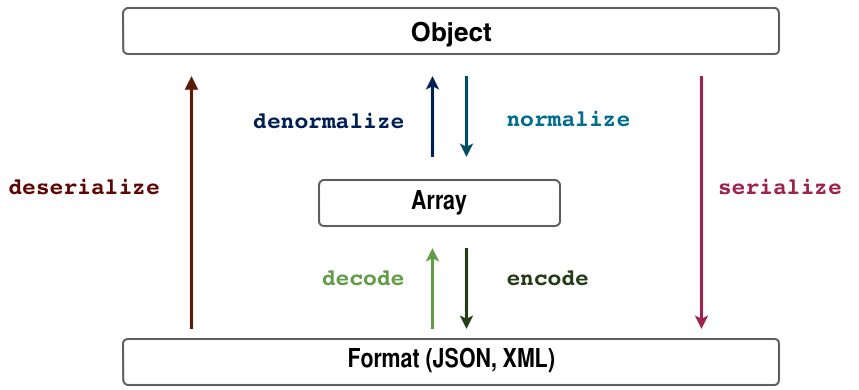
\includegraphics[scale=0.3]{img/serializer_workflow}
    \caption{Diagrama del proceso de serialización de un objeto}
    Fuente: \url{https://symfony.com/doc/current/components/serializer.html}
\end{figure}

Además, mediante el uso de anotaciones, se pueden crear grupos de
serialización, de forma que dependiendo de la petición recibida se pueden
serializar distintos atributos. En el siguiente ejemplo se crean tres grupos,
\textit{private}, \textit{public} y \textit{edit}:

\begin{minted}[linenos=true]{php}
<?php

use Doctrine\ORM\Mapping as ORM;
use Symfony\Component\Serializer\Annotation\Groups;
use Symfony\Component\Validator\Constraints as Assert;

/**
 * @ORM\Entity
 */
class House
{
    /**
     * @ORM\Id()
     * @ORM\GeneratedValue()
     * @ORM\Column(type="integer")
     *
     * @Groups({"private"})
     */
    private $id;

    /**
     * @ORM\Column(type="string", length=255)
     *
     * @Assert\NotBlank()
     * @Assert\Length(min = 1, max = 255)
     *
     * @Groups({"public", "edit"})
     */
    private $name;

    /**
     * @ORM\Column(type="integer")
     *
     * @Assert\GreaterThanOrEqual(0)
     *
     * @Groups({"public"})
     */
    private $stories;
}
\end{minted}

Habiendo etiquetado cada atributo en uno o más grupos de serialización, esto
después puede utilizarse para gestionar de forma dinámica la entidad
dependiendo de las peticiones. Por ejemplo, cuando se hiciera únicamente una
operación de lectura por parte de un cliente sin privilegios, la entidad podría
ser serializada con el grupo \textit{public}, dejando así el atributo
\textit{id} fuera de la respuesta a dar. Lo mismo aplica para los grupos
\textit{edit} que podría utilizarse para limitar las modificaciones a un
atributo en concreto, o el grupo \textit{private} si la casa está siendo
gestionada por un administrador. Los grupos de los nombres en este caso son
esos, pero pueden llamarse como se quiera.

\subsubsection{behat/behat}
Un \glslink{webframework}{framework} \gls{bdd} que permite realizar
\glslink{testsfuncionales}{pruebas funcionales} mediante una sintaxis denominada
\textit{Gherkin}, que facilita la redacción y lectura de las pruebas.
Dichas pruebas se organizan en funcionalidades, escenarios y pasos que después
el \glslink{webframework}{framework} se encarga de ejecutar. Un ejemplo de una
prueba funcional con esta librería podría ser el siguiente:

\begin{minted}[linenos=true]{gherkin}
Feature: House management
  In order to manage houses
  As a house owner
  I need to be able to add a house, modify its parameters or remove it

  Scenario: Modify a house
    Given there exists a house named "My fancy house"
    And I am the owner of it
    When I modify its name to "My beautiful house"
    Then its new name should be "My beautiful house"
\end{minted}

Esta definición de la prueba funcional en \textit{Gherkin} después se mapea a
una clase \gls{php} que interpreta y ejecuta lo que en cada paso debe de
comprobarse:

\begin{minted}[linenos=true]{php}
<?php

class FeatureContext
{
    /**
     * @Given there exists a house named :house
     */
    public function thereExistsHouseNamed($house)
    {
      if(!exists_house($house)) {
        throw new Exception(
          'The house ' . $house . ' doesn't exist'
        );
      }
    }

    /**
     * @Given I am the owner of it
     */
    public function iAmTheOwnerOfTheHouse()
    {
      /** Do stuff */
    }

    /**
     * @When I modify its name to :newName
     */
    public function iModifyItsNameTo($newName)
    {
      /** Do stuff */
    }

    /**
     * @Then its new name should be :expectedName
     */
    public function theNewNameShouldBe($expectedName)
    {
      /** Do stuff */
    }
}
\end{minted}
Este ejemplo se ha simplificado para facilitar la asimilación del concepto
detrás de \textit{Behat}. Una vez hechos los mapeos correctamente
\textit{Behat} se encargará de ejecutar las funciones, y en caso de que no
produzcan ningún error los pasos correspondientes se considerarán como
correctos.

\subsubsection{justinrainbow/json-schema}
Librería utilizada para validar objetos JSON con \textit{JSON Schema}. Por
ejemplo, imaginemos que al realizar una petición al servidor para
obtener información sobre una entidad \textit{House}, dicho servidor devuelve
lo siguiente:
\begin{minted}[linenos=true]{json}
{
  "id": 1,
  "name": "My beautiful house",
  "stories": 2
}
\end{minted}
A la hora de realizar las pruebas de la aplicación, la información que devuelva
el servidor puede ser variada, a pesar de que el entorno de pruebas cargue una
serie de casas predefinidas. En vez de validar que el JSON que devuelve el
servidor es exactamente igual a las diferentes casas que existen en la base de
datos \textemdash porque recordemos que en vez de devolver un único objeto
\textit{House}, el servidor podría devolver un \textit{array} de ellos
\textemdash, se puede comprobar que el objeto JSON devuelto es válido acorde a
un esquema. Por ejemplo:

\begin{minted}[linenos=true]{json}
{
  "type": "object",
  "properties": {
    "id": {"type": "integer"},
    "name": {
      "type": "string",
      "pattern": "^[a-zA-Z0-9]+$"
    },
    "stories": {
      "type": "integer",
      "minimum": 0
    }
  },
  "required": ["id", "name"]
}
\end{minted}
Este esquema, que ha obviado algunos elementos para simplificar el ejemplo,
podría utilizarse para validar las diferentes respuestas que puede dar el
servidor con respecto a diferentes casas. Esto puede resultar muy interesante
para reducir el tamaño de las pruebas y concentrar en un único esquema las
condiciones del objeto JSON que el servidor debería de enviar.

\subsubsection{lexik/jwt-authentication-bundle}
Esta librería provee de una implementación de los \gls{jwt}: Esta tecnología
es un estándar abierto\footnote{\url{https://tools.ietf.org/html/rfc7519}} que
define una forma compacta y autocontenida \textemdash debido a que el token
tiene toda la información del usuario y no es necesario volver a consultar a la
base de datos \textemdash de intercambiar
información entre dos entidades mediante un objeto JSON. Además, la información
puede ser verificada debido a que se firma digitalmente bien utilizando un
secreto, bien utilizando claves públicas y privadas. \cite{jwt_explanation}

Como se ha comentado anteriormente, \gls{jwt} tiene una naturaleza compacta y
autocontenida. Esto es realmente útil, por ejemplo, en arquitecturas \gls{rest}
donde no hay estados: debido a que cada llamada a una \gls{api} \gls{rest} debe
de contener toda la información necesaria para que el servidor pueda procesarla
correctamente, los tokens \gls{jwt} son extremadamente útiles para transmitir,
por ejemplo, la información respecto al usuario que está realizando dicha
llamada. De esta forma el servidor puede extraer todos los datos del token para
comprobarlos y autorizar o no el procesamiento de la petición realizada. He
aquí un diagrama explicando el proceso de inicio de sesión:

\begin{figure}[h]
    \center
    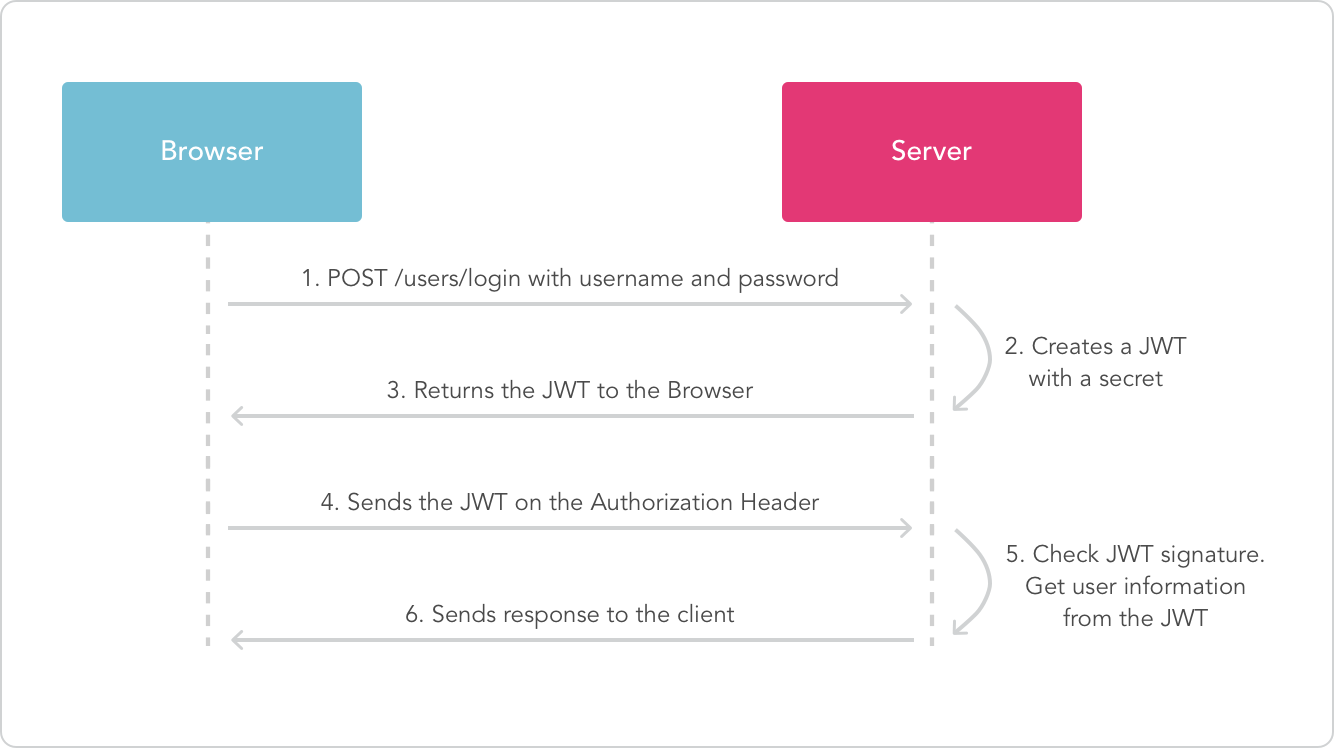
\includegraphics[scale=0.2]{img/jwt-diagram}
    \caption{Diagrama del proceso de inicio de sesión mediante un token
      \textit{JWT}.}
    Fuente: \url{https://jwt.io/introduction/}
\end{figure}

Tal y como se ve en el diagrama, el token \gls{jwt} se envía adjuntado en cada
petición, en una de las cabeceras de la misma: la cabecera
\textit{Authorization}.

\subsubsection{api-platform/api-pack}
Este es un metapaquete el cual agrupa otras librerías que dan la funcionalidad
necesaria para incorporar API Platform en una instalación estándar de Symfony.
Entre otras librerías, incluye \textit{api-platform/core}, que es la librería
que al fin y al cabo provee de las funcionalidades indicadas en la sección de
\glslink{webframework}{frameworks} \ref{tech:apiplat}.
